\section{Obtención de conjunto de datos}


La obtención del conjunto de datos se divide en dos etapas, la primera etapa corresponde a la toma de muestras, la cual implica ir al lugar con flujo constante de vehículos para obtener la mayor cantidad de datos. La segunda etapa es la limpieza de las muestras con la cual se busca solo tomar en cuenta los vehículos a los que se logró tomar correctamente la velocidad.
La Figura \ref{fig:DFCreacionCD} muestra las dos etapas internas con las que cuenta la obtención de conjunto de datos.

\begin{figure}[H]
    \centering
    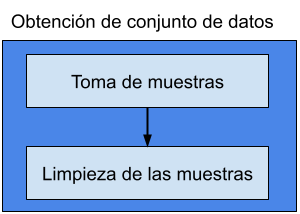
\includegraphics[width=0.5\textwidth]{Metodologia/imgs/ObtencionConjuntoDatos.png}
    \caption{Proceso de obtención de conjunto de datos.}
    \label{fig:DFCreacionCD}
\end{figure}


%%%%%%%%%%%%%%%%%%%%%%%%%%%%%%%%%%%%%%%%%%%%%%%%%%%%%%%%%%%%%%%%%%%%%%%%%%%%%%%%
%%%%%%%%%%%%%%%%%%%%%%%%%%%%%%%%%%%%%%%%%%%%%%%%%%%%%%%%%%%%%%%%%%%%%%%%%%%%%%%%
%%%%%%%%%%%%%%%%%%%%%%%%%%%%%%%%%%%%%%%%%%%%%%%%%%%%%%%%%%%%%%%%%%%%%%%%%%%%%%%%
%%%%%%%%%%%%%%%%%%%%%%%%%%%%%%%%%%%%%%%%%%%%%%%%%%%%%%%%%%%%%%%%%%%%%%%%%%%%%%%%
%%%%%%%%%%%%%%%%%%%%%%%%%%%%%%%%%%%%%%%%%%%%%%%%%%%%%%%%%%%%%%%%%%%%%%%%%%%%%%%%

\subsection{Toma de muestras}

Para la toma de muestras se requirió de dos dispositivos con los cuales se busca la extracción del conjunto de datos que posteriormente se utilizará como entrenamiento de los modelos predictivos. Uno de los dispositivos es el radar Bushnell (Figura \ref{fig:RadarVelocidad}) el cual tiene una precisión de +/- 1.6 kilómetros por hora.

\begin{figure}[H]
    \centering
    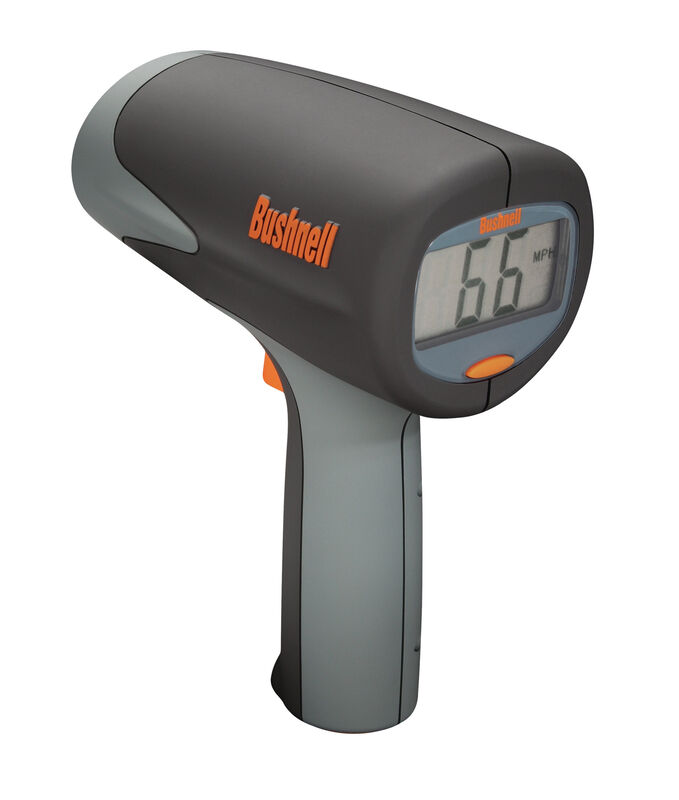
\includegraphics[width=0.4\textwidth]{Metodologia/imgs/bushnell.jpg}
    \caption{Radar de velocidad Bushnell(\cite{bushnell}).}
    \label{fig:RadarVelocidad}
\end{figure}

Mientras que el otro dispositivo es una cámara de video, la cual puede ser un dispositivo especializado para esta tarea o cualquier otro dispositivo capaz de grabar video. 
Las configuraciones mínimas pueden ser una resolución de 854 x 480 a 30 fotogramas por segundo. Sin embargo, hay que tomar en cuenta que al tener una resolución baja se puede perder calidad en la imagen y tomar un área menor a la deseada. Mientras que tener fotogramas tan bajos ocasionará perder vehículos que pasan a una velocidad más alta.
Por otro parte al aumentar la resolución y los fotogramas por segundo ocasiona que al sistema le tome más tiempo procesar el video. Para este caso se utilizó la cámara de Smartphones un Xiaomi Redmi Note 7 y un iPhone X configurados a 60 FPS y una resolución de Full HD (1920 x 1080 pixeles).

Existe un cuidado especial a la hora de posicionar la cámara, ya que no se quiere que los experimentos sean considerados como cálculos de velocidad en 2D, para esto la toma de muestras se realizó en un lugar donde el tráfico vehicular pase con cierto grado de inclinación, sin apuntar la cámara directamente al costado de donde pasan los vehículos, como muestra la Figura \ref{fig:LugarMuestrasDataset}.

\begin{figure}[H]
    \centering
    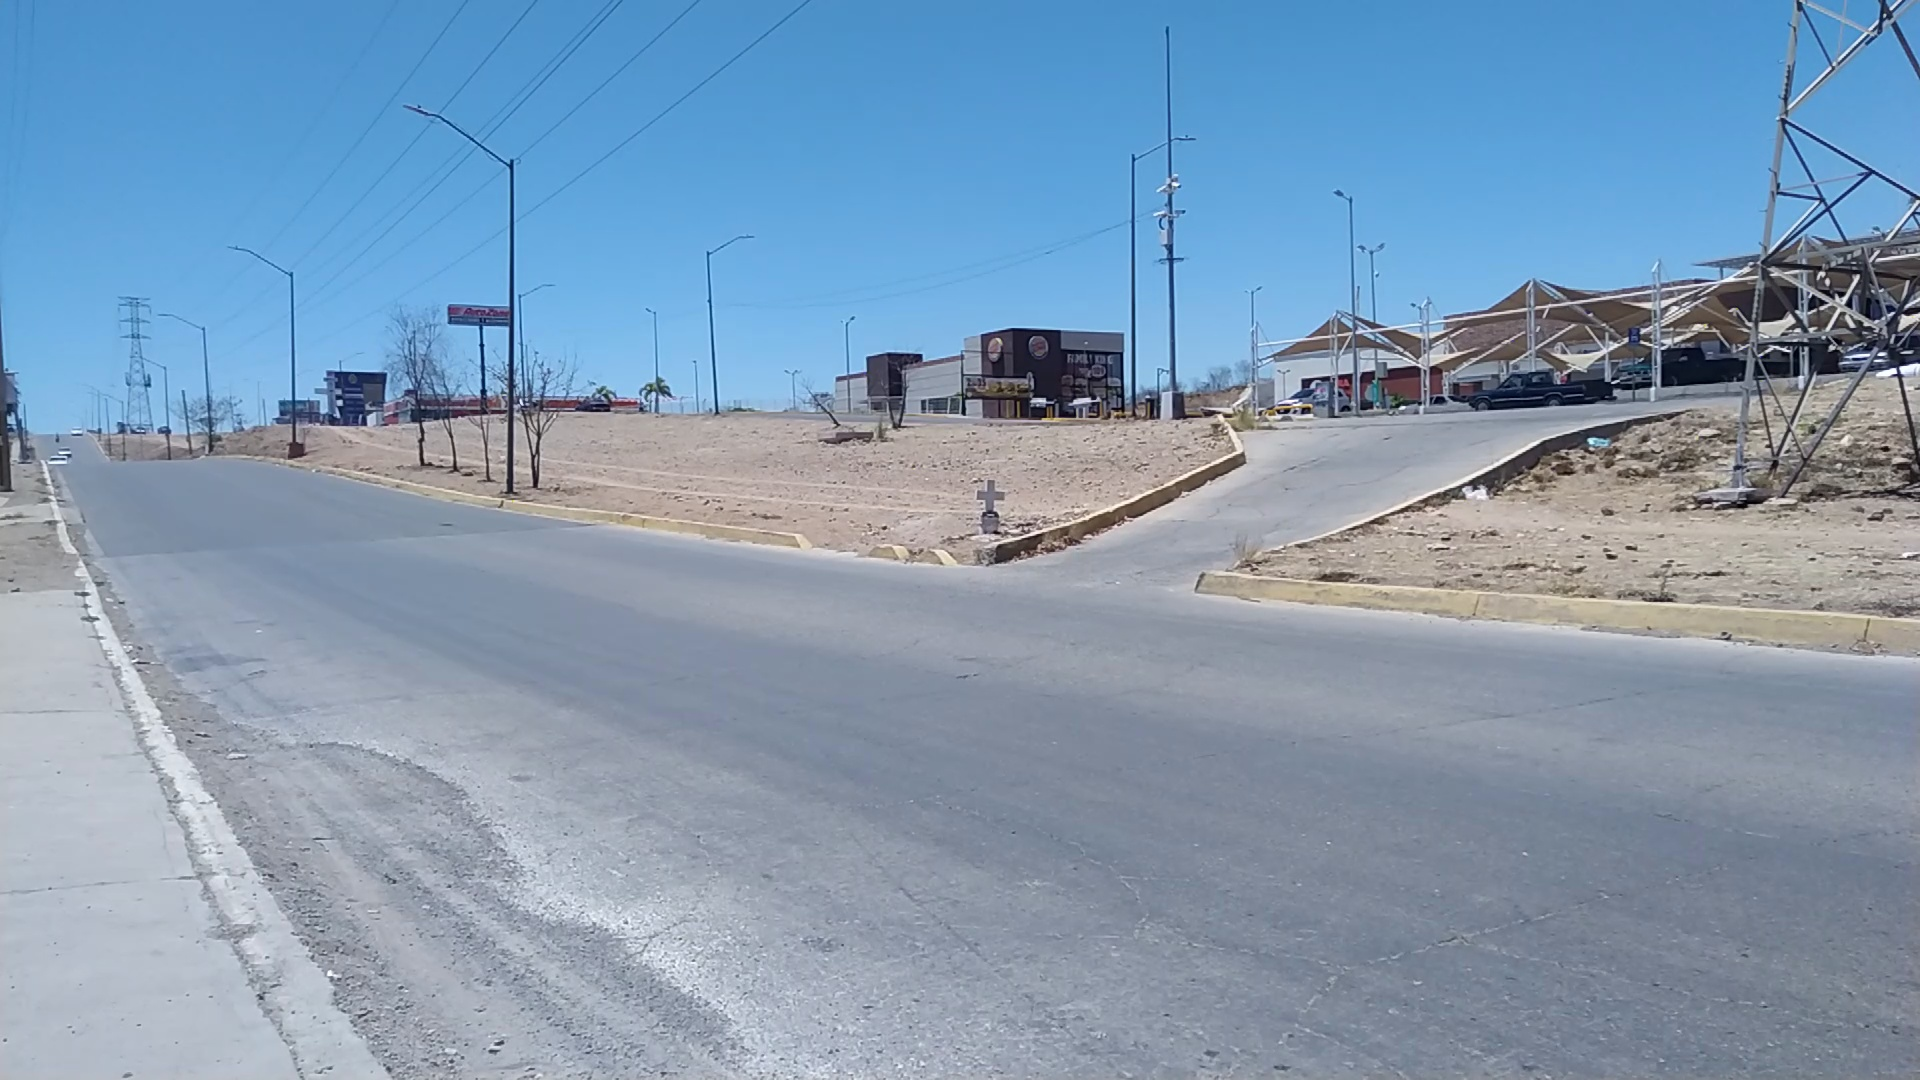
\includegraphics[width=0.8\textwidth]{Metodologia/imgs/LugarMuestras.jpg}
    \caption{Lugar donde se tomaron las muestras.}
    \label{fig:LugarMuestrasDataset}
\end{figure}

Cabe mencionar que por practicidad, el proceso de toma de muestras fue realizado, en un mismo lugar de la ciudad de Culiacán, Sinaloa.

Dado que la cámara y el radar de velocidad son dispositivos que no están sincronizados entre sí, fue necesario la implementación de un mecanismo para asociar la lectura del radar con la toma del video.

%%%%%%%%%%%%%%%%%%%%%%%%%%%%%%%%%%%%%%%%%%%%%%%%%%%%%%%%%%%%%%%%%%%%%%%%%%%%%%%%
%%%%%%%%%%%%%%%%%%%%%%%%%%%%%%%%%%%%%%%%%%%%%%%%%%%%%%%%%%%%%%%%%%%%%%%%%%%%%%%%
%%%%%%%%%%%%%%%%%%%%%%%%%%%%%%%%%%%%%%%%%%%%%%%%%%%%%%%%%%%%%%%%%%%%%%%%%%%%%%%%
%%%%%%%%%%%%%%%%%%%%%%%%%%%%%%%%%%%%%%%%%%%%%%%%%%%%%%%%%%%%%%%%%%%%%%%%%%%%%%%%
%%%%%%%%%%%%%%%%%%%%%%%%%%%%%%%%%%%%%%%%%%%%%%%%%%%%%%%%%%%%%%%%%%%%%%%%%%%%%%%%

\subsection{Limpieza de las muestras}

Una vez tomadas las muestras, fue necesario realizar una limpieza de los datos, estos son, los vehículos a los que se les detectó la velocidad utilizando el radar. Con la limpieza de los datos se busca eliminar los vehículos a los que no se les tomo la velocidad y dejando solo aquellos que si fueron considerados.

La toma de las muestras se realizá a partir de dos dispositivos que no están especializados para esta tarea (Cámara de video y radar de velocidad), la limpieza de las muestras ayuda a combinar la información de ambos dispositivos realizando una inspección visual de los videos, en la cual se identifica el segundo del video en el que pasa el vehículo de interes, la velocidad detectada por el radar, el carril por el cual viaja el vehículo y una descripción del vehículo para futuras referencias. Estos cuatro datos son guardados en un archivo de texto separado por comas (csv) el cual servirá de entrada para el siguiente paso en la metodología.

Determinar la velocidad es una tarea que necesita el tiempo y la distancia que toma un vehículo en pasar de un lugar a otro. Para esto el sistema necesita ser configurado con un punto de entrada y un punto de salida en el eje X. A partir de ahora a estos dos puntos se les llamará simplemente por punto A y punto B.  Los puntos A y B deben ser colocados de manera que los vehículos deben pasar completamente por cada uno de ellos. Además, cada una de las muestras deben tener diferentes valores para los puntos A y B, sin embargo, para este caso no fue necesario implementar diferentes valores, ya que todos los videos fueron tomados en el mismo lugar. La Figura \ref{fig:LugarLimites} muestra donde fueron colocados los puntos A y B en las muestras, denotados por dos lineas azules verticales.

\begin{figure}[H]
    \centering
    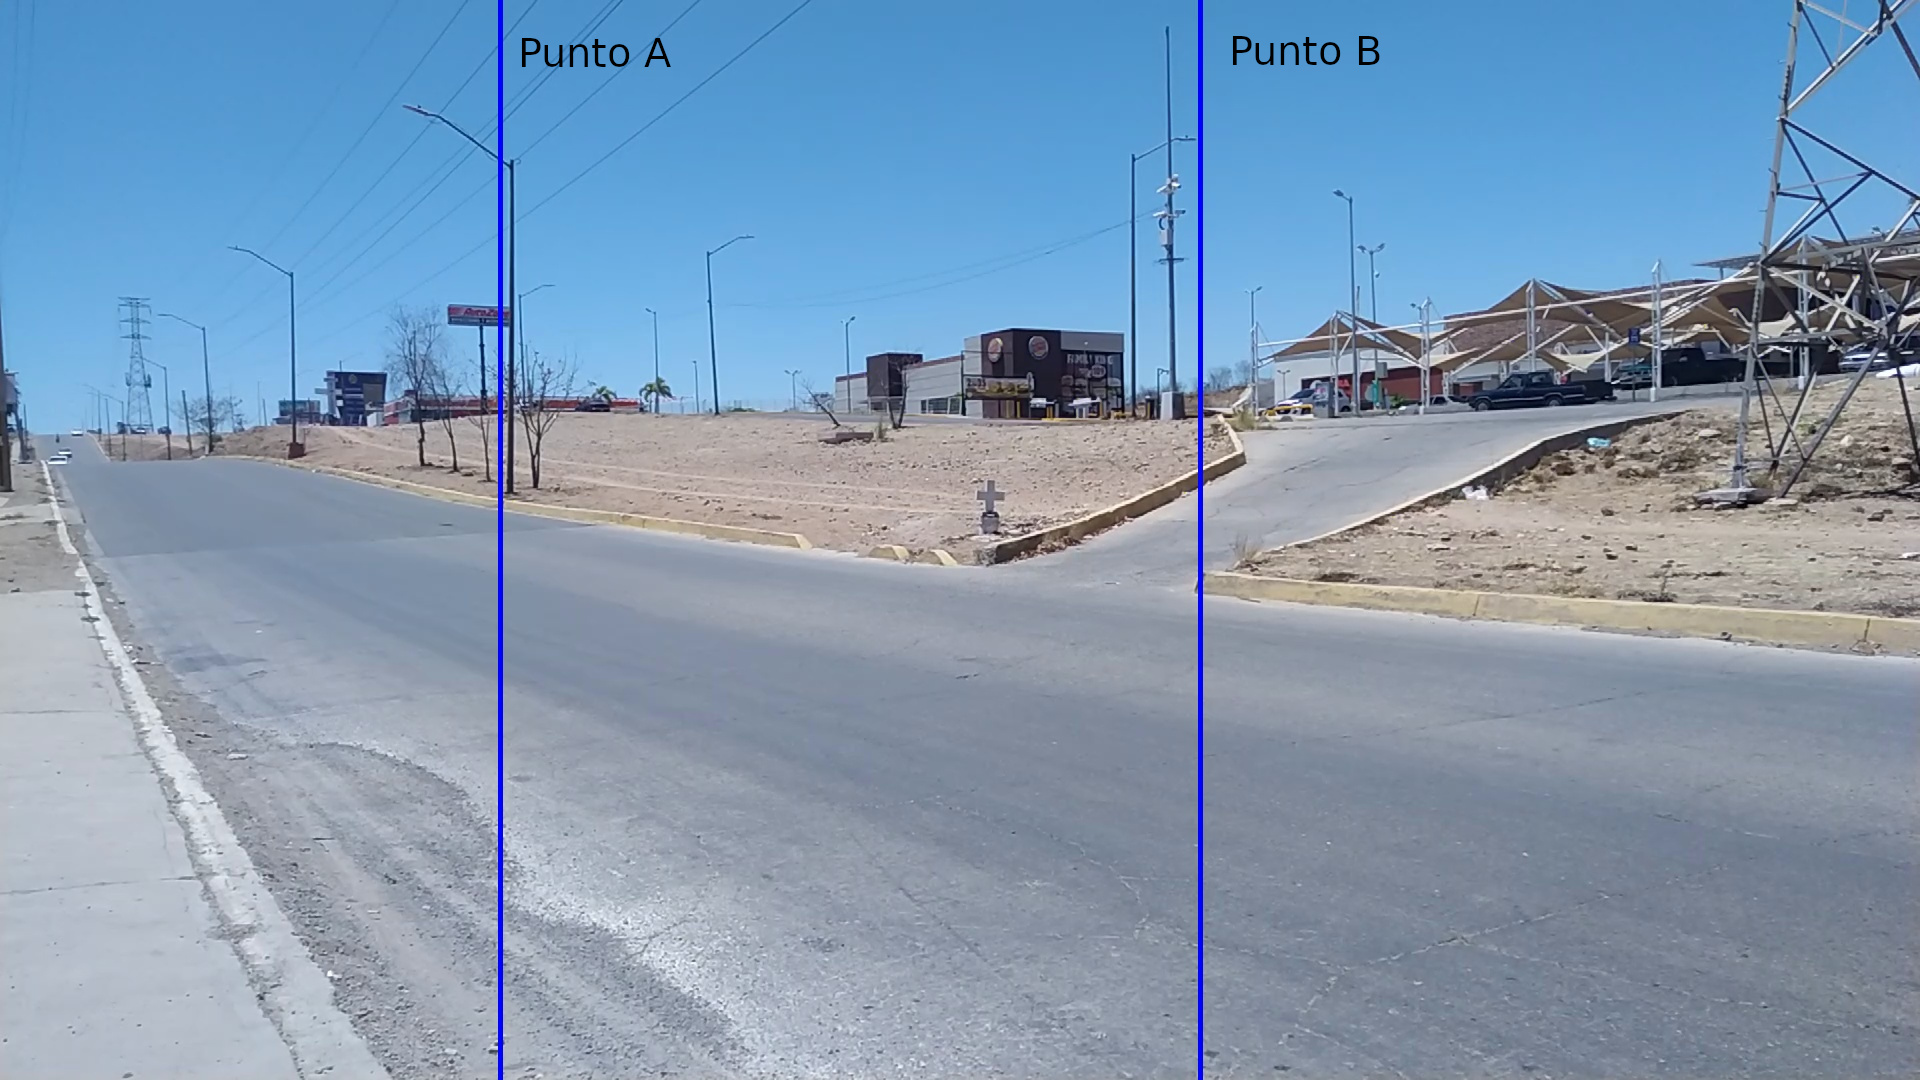
\includegraphics[width=0.8\textwidth]{Metodologia/imgs/LugarLimites_01.jpg}
    \caption{Límites para lugar de las muestras.}
    \label{fig:LugarLimites}
\end{figure}

Una vez que se deciden los valores para los puntos A y B, se genera el archivo csv. Para esto se toma en cuenta el segundo en que pasa debe ser lo más cercano posible al centroide del vehículo cuando pasa por el punto B. Es importante ingresar una descripción, aunque esta no va a ser usada por el sistema. Se volverá importante para validar que el vehículo al que se le tomó la velocidad es el mismo que detecto el sistema.

%%%%%%%%%%%%%%%%%%%%%%%%%%%%%%%%%%%%%%%%%%%%%%%%%%%%%%%%%%%%%%%%%%%%%%%%%%%%%%%%
%%%%%%%%%%%%%%%%%%%%%%%%%%%%%%%%%%%%%%%%%%%%%%%%%%%%%%%%%%%%%%%%%%%%%%%%%%%%%%%%
%%%%%%%%%%%%%%%%%%%%%%%%%%%%%%%%%%%%%%%%%%%%%%%%%%%%%%%%%%%%%%%%%%%%%%%%%%%%%%%%
%%%%%%%%%%%%%%%%%%%%%%%%%%%%%%%%%%%%%%%%%%%%%%%%%%%%%%%%%%%%%%%%%%%%%%%%%%%%%%%%
%%%%%%%%%%%%%%%%%%%%%%%%%%%%%%%%%%%%%%%%%%%%%%%%%%%%%%%%%%%%%%%%%%%%%%%%%%%%%%%%
